% Generated by code/needham.py -- do not edit by hand.
\definecolor{qocA}{rgb}{0.00,0.45,0.70}
\definecolor{qocB}{rgb}{0.90,0.60,0.00}
\definecolor{qocC}{rgb}{0.00,0.62,0.45}
\definecolor{qocD}{rgb}{0.80,0.40,0.00}
\definecolor{qocE}{rgb}{0.80,0.60,0.70}
\definecolor{qocF}{rgb}{0.35,0.70,0.90}
\begin{tikzpicture}[ink/.style={line width=0.9pt, ndInk}, faint/.style={line width=0.4pt, ndInk!35}, dashedink/.style={line width=0.5pt, ndInk!55, dash pattern=on 2.5pt off 2pt}, vec/.style={->, >=stealth, line width=1.2pt}, note/.style={font=\footnotesize\itshape, text=ndInk!85, align=center}, pointer/.style={->, >=stealth, line width=0.4pt, ndInk!60, shorten >=2pt, shorten <=1pt}, dot/.style={circle, fill=ndInk, inner sep=0pt, minimum size=3.4pt}, wash/.style={fill=ndSky, fill opacity=0.55}, every node/.style={text=ndInk}]
\definecolor{ndInk}{rgb}{0.13,0.13,0.18}
\definecolor{ndPaper}{rgb}{0.99,0.96,0.88}
\definecolor{ndSky}{rgb}{0.84,0.91,0.98}
\definecolor{ndRose}{rgb}{0.98,0.86,0.84}
\definecolor{ndBlue}{rgb}{0.13,0.36,0.66}
\definecolor{ndRed}{rgb}{0.78,0.20,0.16}
\definecolor{ndGold}{rgb}{0.88,0.62,0.10}
\definecolor{ndGreen}{rgb}{0.18,0.52,0.30}
\draw[dashedink] (0,0) circle (2.694);
\fill[ndRose, fill opacity=0.35] (0,0) circle (2.694);
\fill[ndSky] (2.333,1.347) -- (-2.333,1.347) -- (0.000,-2.694) -- cycle;
\draw[line width=1.4pt, ndBlue] (2.333,1.347) -- (-2.333,1.347) -- (0.000,-2.694) -- cycle;
\draw[line width=0.8pt, ndGreen] (0,0) circle (1.347);
\draw[faint, ->, >=stealth] (-3.13,0) -- (3.13,0) node[right] {$x_3$};
\draw[faint, ->, >=stealth] (0,-3.13) -- (0,3.13) node[above] {$x_8$};
\node[dot, fill=ndBlue, label={[font=\footnotesize]above right:$\ket0\bra0$}] at (2.333,1.347) {};
\node[dot, fill=ndBlue, label={[font=\footnotesize]above left:$\ket1\bra1$}] at (-2.333,1.347) {};
\node[dot, fill=ndBlue, label={[font=\footnotesize]below:$\ket2\bra2$}] at (0.000,-2.694) {};
\node[dot, fill=ndGreen] at (0.000,1.347) {};
\node[dot, fill=ndGreen] at (-1.167,-0.674) {};
\node[dot, fill=ndGreen] at (1.167,-0.674) {};
\node[dot, fill=ndInk!60, label={[font=\scriptsize]below right:$\tfrac13\Id$}] at (0,0) {};
\node[dot, fill=ndRed, minimum size=4.2pt] at (0.000,2.640) {};
\draw[->, >=stealth, line width=0.7pt, ndRed] (0,0) -- (0.000,2.570);
\node[note, anchor=west, text=ndBlue] (a) at (3.53,1.9) {states in this slice:\\ a \emph{triangle}, corners pure};
\draw[pointer] (a.west) to[bend right=15] (1.810,0.367);
\node[note, anchor=west] (o) at (3.53,0.6) {outer circle $\norm{\vec x}=\sqrt{2/3}$:\\ touched only at the pure states};
\draw[pointer] (o.west) to[bend left=10] (2.675,0.323);
\node[note, anchor=west, text=ndGreen!70!black] (i) at (3.53,-0.7) {inner circle $\norm{\vec x}=1/\sqrt6$:\\ touched at the midpoints};
\draw[pointer] (i.west) to[bend left=15] (1.247,-0.724);
\node[note, anchor=east, text=ndRed] (r) at (-1.48,3.13) {$0.8\,F_8$: inside the outer\\circle, but not a state\\ (negative eigenvalue):\\ no symmetry $\vec x\mapsto-\vec x$};
\draw[pointer] (r.east) to[bend left=15] (-0.100,2.660);
\end{tikzpicture}
